\subsubsection{Kommunikationsmodul}
\begin{figure}[h]
\centering
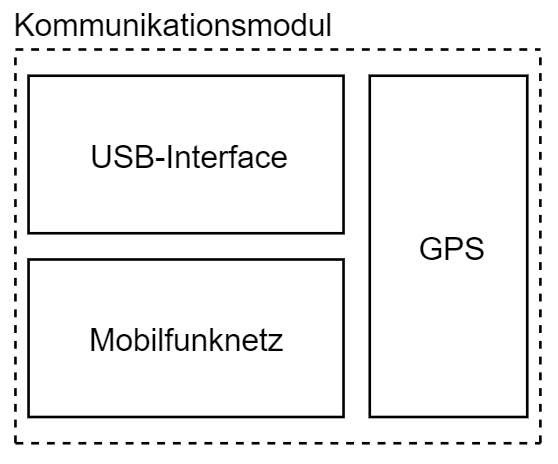
\includegraphics[scale=0.7]{graphics/Konzeptdiagramme/Kommunikationsmodul.PNG}
\caption{Kommunikationsmodul}
\label{fig:kommunikationsmodul}
\end{figure}
Abbildung \ref{fig:kommunikationsmodul} zeigt die verschiedenen Schnittstellen, über welche Daten mit der Umgebung (User) und \textit{MCU} ausgetauscht werden können. Im Rahmen des Projekts 5 wurde das USB-Interface umgesetzt. Mobilfunknetz und GPS sind Teil des Projekts 6.\\

\subparagraph{USB-Interface:}
Über dieses Interface kann mit dem System kommuniziert und interagiert werden. Ein serielles Terminal-Emulationsprogramm (wie z.B. PuTTY) wird dazu benötigt.\\

\subparagraph{Mobilfunknetz:}
Die Einbindung der Wetterstation wird über diesen Block implementiert. Dazu wird ein GSM-Modul benötigt.\\

\subparagraph{GPS:}
Dieser Block sorgt für die Standortbestimmung. Dafür wird ein GPS-Modul auf dem PCB integriert.\\